% Abstract page (ii), per "3. Abstract": the project record block, the word
% "Abstract" centred, the text, and keywords sorted A-Z.  The abstract states
% what was done and what was found at the reporting cutoff; it does not
% anticipate the four real-robot slots that are still planned.
\thispagestyle{report}
\phantomsection\addcontentsline{toc}{chapter}{ABSTRACT}
\noindent
\begin{tabular}{@{}p{0.24\textwidth}p{0.73\textwidth}@{}}
Project Title & Vision-Based Navigation Pipeline for AMRs in a Dynamic Warehouse \\
Project Credits & 6 \\
Candidate & Mr.\ Bolton Athit Davies \\
Project Advisor & Dr.\ Rattanachai Ramaithitima \\
Program & Bachelor of Engineering \\
Field of Study & Robotics and Automation Engineering \\
Faculty & Institute of Field Robotics \\
Academic Year & 2026 \\
\end{tabular}

\vspace{10mm}
\begin{center}Abstract\end{center}
\vspace{2mm}

Autonomous mobile robots in warehouses are today navigated with 2-D LiDAR and
QR-code infrastructure, which is costly to install and inflexible when the
warehouse changes. This project develops and evaluates a vision-based navigation
pipeline in which a stereo-inertial visual SLAM front end is combined with a
YOLO object detector that removes image features belonging to movable warehouse
objects before they enter pose estimation. Two pipelines are compared:
ORB-SLAM3 with detector-driven feature rejection, and VINS-Fusion with
persistent-track culling feeding an RTAB-Map mapping back end. The work is
organised as four experiments, each defined for both a Gazebo simulation of the
warehouse and the real robot: a non-visual baseline and estimator comparison, an
offline evaluation of the detector, a visual-inertial odometry evaluation with
dynamic-environment filtering, and a dense-map reconstruction and map-quality
evaluation.

At the reporting cutoff the four simulation experiments have been run and the
four real-robot experiments remain planned. On five static recordings a
five-state wheel-plus-gyroscope extended Kalman filter localises to
\SIrange{0.19}{0.49}{\metre} aligned ATE, ahead of both visual pipelines as
configured, but that ordering reverses on every recording once the filter is
given the visual systems' own inertial noise model; the noise model, not the
architecture, dominates. All three dead-reckoning estimators are overconfident
by about two orders of magnitude. The detector reaches a pooled precision of
0.684 and a moving-object recall of 0.591 against projected simulator ground
truth, with conditional class accuracy of 0.996. The dynamic-filtering
hypothesis remains untested: the VINS-Fusion filter never activated, the
ORB-SLAM3 treatment pairs were not input-matched, and the scripted dynamic
worlds were found not to constitute a valid testbed. The RTAB-Map map of the
small warehouse is geometrically faithful (occupied-cell precision 96.6\%,
observed-surface recall 89.5\%) and drivable along an independent route; the
large-warehouse map failed through tracking loss under repetitive structure.
The report records these outcomes with their validity limits and sets out the
remaining plan.

\vspace{6mm}
\noindent Keywords: Autonomous Mobile Robot / Dynamic Environment /
Extended Kalman Filter / Object Detection / ORB-SLAM3 / RTAB-Map / Visual SLAM /
VINS-Fusion / YOLO
\clearpage

% Thai abstract (iii).  pdflatex has no Thai font on this host, so the page is
% typeset by LibreOffice from frontmatter/thai_abstract.fodt (Norasi 16 pt, the
% installed stand-in for AngsanaUPC 16 pt, same 4/2/3/2 cm margins) and placed
% here as a PDF page; script/build_final_report.sh regenerates it.
\phantomsection\addcontentsline{toc}{chapter}{THAI ABSTRACT}
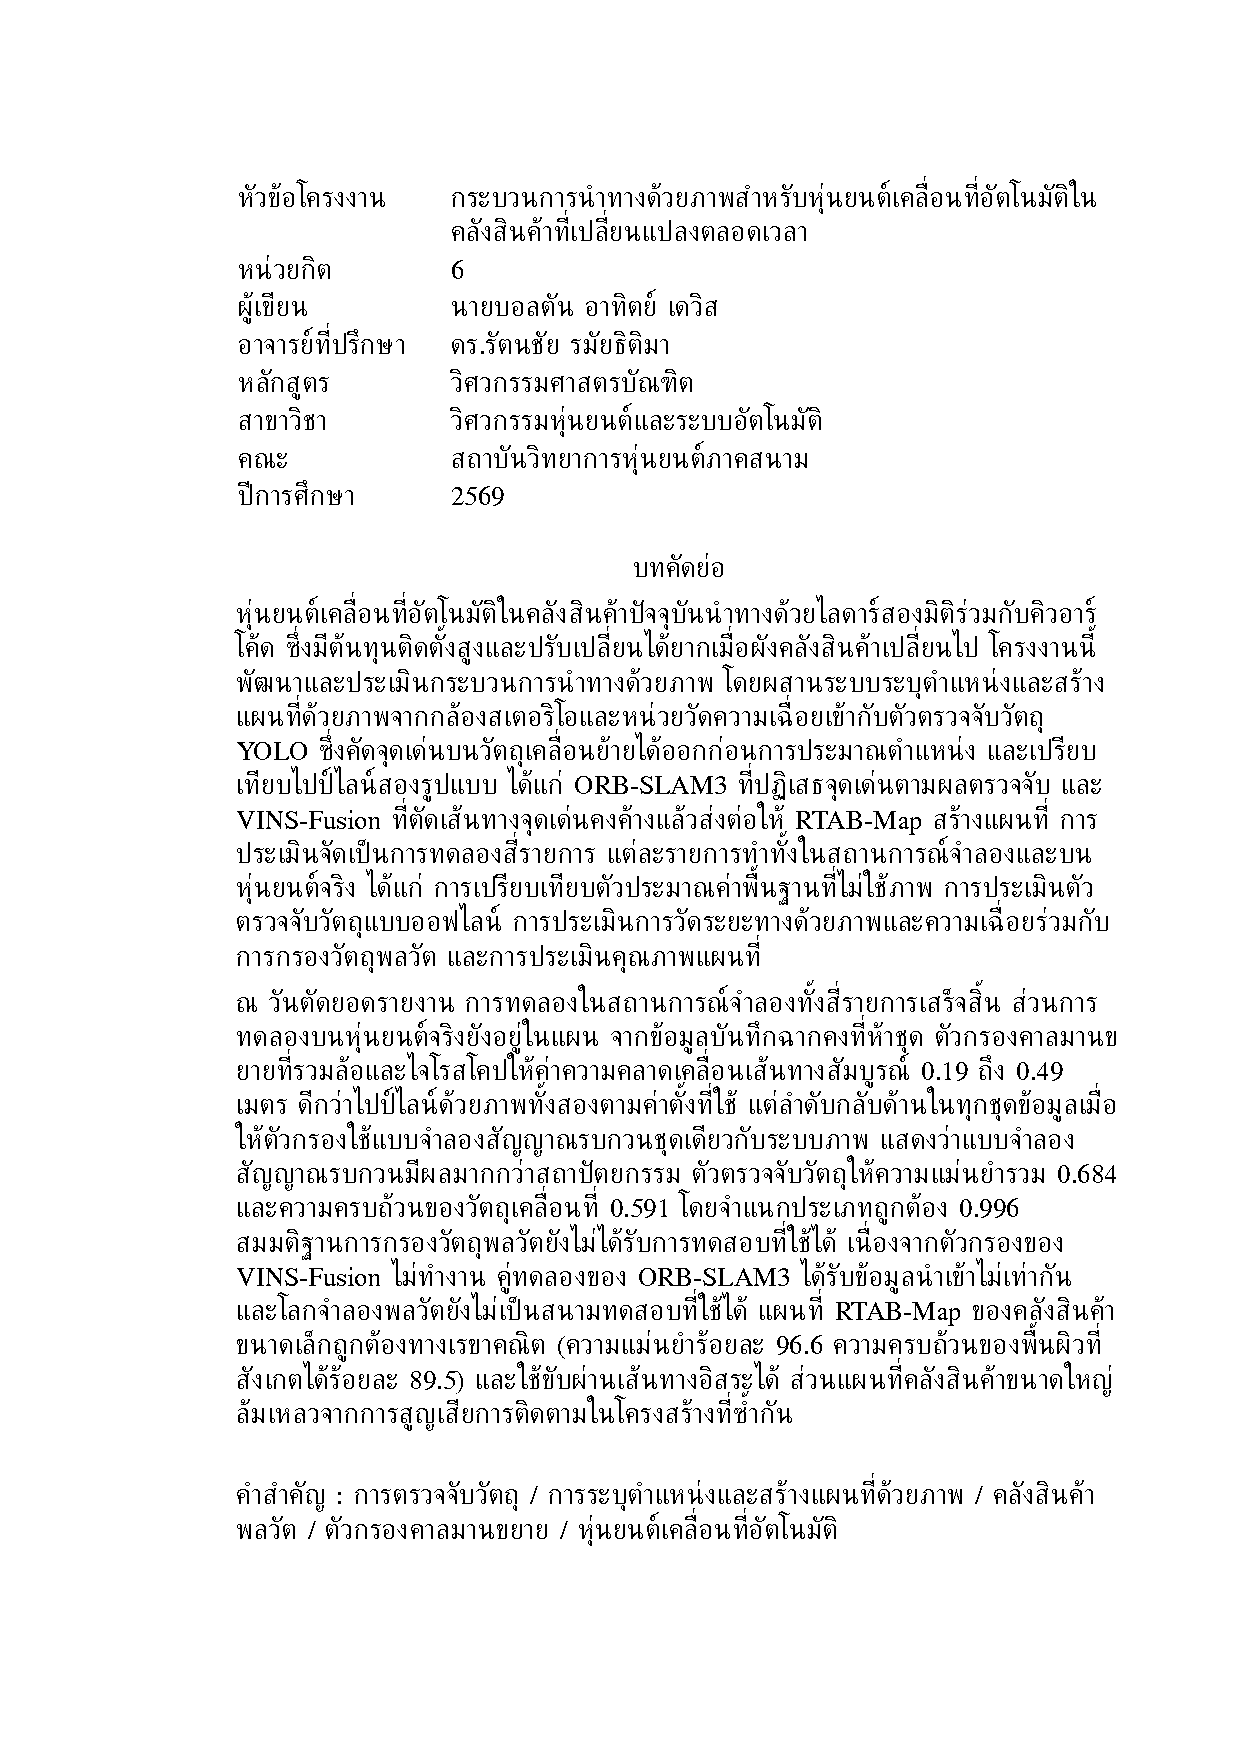
\includepdf[pages=1, pagecommand={\thispagestyle{report}}]{frontmatter/thai_abstract.pdf}
